\section{Background Theory}

\subsection{Software Used}
\subsubsection{OpenWRT Router Software}
OpenWRT is an open-source Linux distribution initially released in 2004 for embedded devices, typically wireless routers. It supports 50 different platforms including AVR32, ARM, PowerPC and X86. It was originally built by Linksys who used it for their WRT54G series of wireless routers.

\subsubsection{SoftEther VPN Bridge}
\label{sec:comms_theory_vpn} % This needs to stay - we refer to here from web. ok
SoftEther VPN Bridge allows you to cascade-connect to a SoftEther VPN Server at a remote location and create an IP Layer-2 bridge connection between the VPN connection and a physical network adapter on the computer running the SoftEther VPN Bridge. It is ideal when all other ports are blocked except normal web service ports as it can tunnel using SSL which bypasses the restrictions. This is invaluable in the case of the university network due to all ports being blocked except 80 (HTTP) and 443 (SSL/HTTPS).

\subsection{Hardware Used}
\subsubsection{Biquad Yagi Antenna}
The Biquad Yagi is a hybrid antenna based on the biquad antenna \ref{fig:biquad} and the Yagi-Uda antenna \ref{fig:yagi} with significantly better properties for our use case than either one. It has very high gain like the Yagi, but maintains a relatively wide beam angle like the biquad. 

\begin{figure}[!htb]
\begin{center}
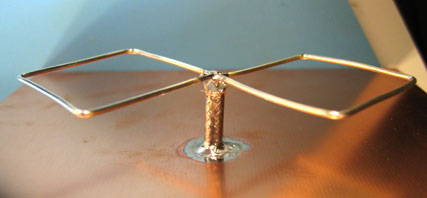
\includegraphics[width=15cm]{bi-quad_side.jpg}
\end{center}
\caption{Biquad Antenna}
\label{fig:biquad}
\end{figure}

\begin{figure}[!htb]
\begin{center}
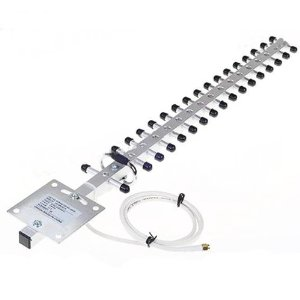
\includegraphics[width=10cm]{yagi.jpg}
\end{center}
\caption{Yagi-Uda Antenna}
\label{fig:yagi}
\end{figure}

%could put an image of the one we use in.
